\subsection{Field study}

Customer for this project, Artsdatabanken, is a Norwegian  Biodiversity Information Center which is devoted to providing public biodiversity information. It keeps species records of birds, insects, and plants among other things. It currently has 6 million registered species, 85\% of which birds\cite{arts:field-study}. \newline

Species are registered individually or in collaboration and in company of two or more individual obervers. Observations / Sightings are a collection of attributes about a species such as name of species, the total number of species, type of species present, and number of each species, activity they were engaged during observation species(resting, feeding, nesting, brooding, passing by), majority number of species, the least/rare species, age, sex, observation start/end date/time, observer, co-observer,and location. Registered data quality is validated by reputation and bibliometric qualities.\newline

\begin{figure}[htb]
	\centering
	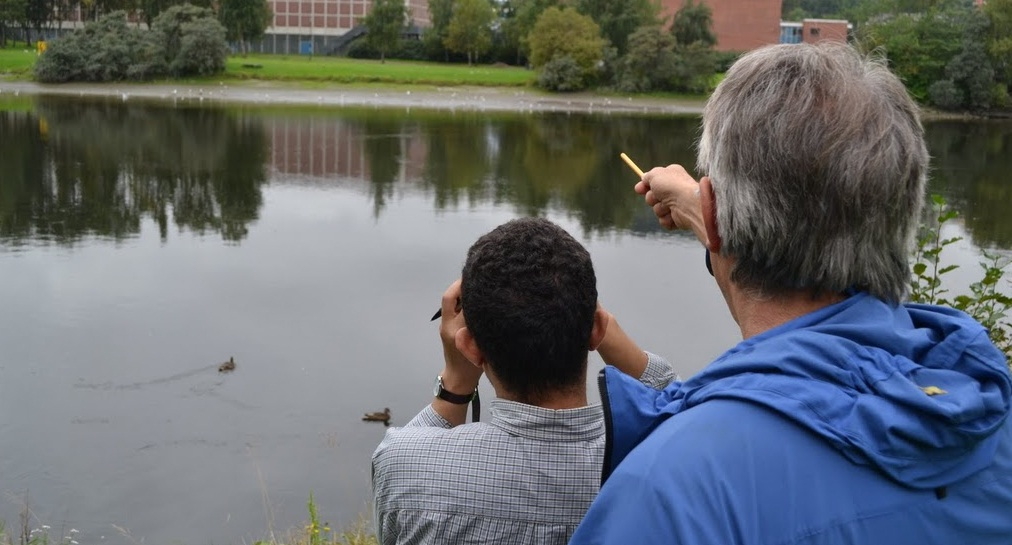
\includegraphics[width=0.8\textwidth]{prestudy/field_study/field_stud.jpg}
	\caption{Counting number of different species}
	\label{fig:field_study}
\end{figure}

Sighting location and species picture are non-negotiable features of the system. Location can be known and already registered or can be conjured up using GPS coordinates. Locations are classified as super and sublocations. Pictures are used based on convenience such as for plants and immobile species candidates.\newline

The customer wants the team to provide full mobility to observers with offline data storage  and synchronization, and also a full comparison of the iOS and Android platform possibilities, and what they stand to gain or lose in adopting the technologies. The customer also suggested keeping all the functionalities of the desktop, and breaking down those functionalities on the mobile device.\newline

During any sighting, the recommendation is to use approximate number of species seen for common species, while being strictly accurate for rare species or not mentioning a number. The customer wants user profiling, type of species that observer wants to report, the total number of species etc.

\begin{figure}[htb]
	\centering
	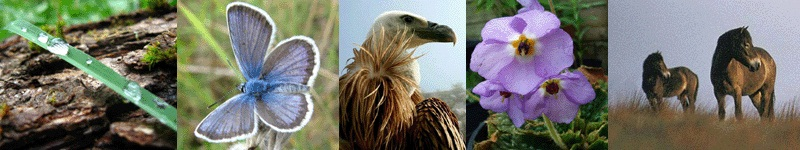
\includegraphics[width=1\textwidth]{prestudy/field_study/flora_fauna_Nikola.jpg}
	\caption{Observation can include rare and endangered species}
	\label{fig:field_study_species}
\end{figure}


